\documentclass{article}
\usepackage[superscript,biblabel]{cite}
\usepackage{graphicx}
\usepackage{float}
\usepackage{threeparttable}
\usepackage{authblk}

\makeatletter
\renewcommand\AB@affilsepx{. \protect\Affilfont}
\makeatother

\graphicspath{{../../analysis/images/}}
\bibliographystyle{naturemag}

\title{Detection and replication of epistasis influencing transcription in humans}
\date{}
\author[1,2,*]{Gibran Hemani}
\author[1,2]{Konstantin Shakhbazov}
\author[3]{Harm-Jan Westra}
\author[4]{Anjali K Henders}
\author[1,2]{Allan F. McRae}
\author[5]{Andres Metspalu}
\author[6]{Greg Gibson}
\author[4]{Nick G Martin}
\author[5,7,8]{Tonu Esko}
\author[3]{Lude Franke}
\author[4]{Grant W Montgomery}
\author[1,2]{Peter M Visscher}
\author[1,2]{Joseph E Powell}

{\tiny

\affil[1]{University of Queensland Diamantina Institute, University of Queensland, Princess Alexandra Hospital, Brisbane, Queensland, Australia}

\affil[2]{The University of Queensland, Queensland Brain Institute, Brisbane, QLD, Australia}

\affil[3]{Department of Genetics, University Medical Center Groningen, University of Groningen, Hanzeplein 1, Groningen, the Netherlands}

\affil[4]{Queensland Institute of Medical Research, Brisbane, Queensland, Australia}

\affil[5]{Estonian Genome Center, University of Tartu, Tartu, 51010, Estonia}

\affil[6]{School of Biology and Centre for Integrative Genomics, Georgia Institute of Technology, Atlanta, Georgia United States of America}

\affil[7]{Divisions of Endocrinology, Children's Hospital, Boston, MA, 02115, US}

\affil[8]{Medical and Population Genetics, Broad Institute, Cambridge, MA, 02142, US}

\affil[*]{Corresponding author: g.hemani@uq.edu.au}

}

\begin{document}

\maketitle


\begin{abstract}

Epistasis is the phenomenon whereby one polymorphism's effect on a trait depends on other polymorphisms present in the genome. The extent to which epistasis influences complex traits \cite{Carlborg2004} and contributes to their variation \cite{Hill2008a, Crow2010} is a fundamental question in evolution and human genetics. Though epistasis has been demonstrated in artificial gene manipulation studies in model organisms \cite{Costanzo2010, Bloom2013}, and some examples have been reported in other species \cite{Carlborg2006}, few convincing examples exist for epistasis amongst natural polymorphisms in human traits \cite{Strange2010, Evans2011}. Its absence from empirical findings may simply be due to its low incidence in the genetic control of complex traits \cite{Hill2008a, Crow2010}, but an alternative view is that it has previously been too technically challenging to detect due to statistical power and computational issues \cite{Cordell2009}. Here we show that, using advanced computation techniques \cite{Hemani2011} and a gene expression study design, many instances of epistasis are found between common single nucleotide polymorphisms (SNPs). In a cohort of 846 individuals with data on 7339 gene expression levels in whole blood, we found 501 significant pairwise epistatic interactions between common SNPs acting on the expression levels of 238 genes ($p < 2.91 \times 10^{-16}$). We tested the discovery interactions for replication in two independent data sets \cite{Metspalu2004, Fehrmann2011}. Three hundred and forty-five interactions had replication interaction $p$-values that were more extreme than the 2.5\% confidence interval of the distribution under the null hypothesis of no epistasis, with 30 significant at a conservative $p < 0.05$ Bonferroni level. There was evidence of functional enrichment for the interacting SNPs, for instance 44 of the genetic interactions are located within 2Mb of regions of known intra-cellular chromosome interactions \cite{Lieberman-Aiden2009} ($p = 1.8 \times 10^{-10}$). Epistatic networks of three SNPs or more influence the expression levels of 129 genes, whereby one \emph{cis}-acting SNP is modulated by several \emph{trans}-acting SNPs. For example MBNL1 is influenced by an additive effect at rs13069559 which itself is masked by \emph{trans}-SNPs on 14 different chromosomes, with nearly identical genotype-phenotype (GP) maps for each \emph{cis}-\emph{trans} interaction. This study presents the first evidence for multiple instances of epistatic genetic effects emerging from natural genetic variation in humans.

\end{abstract}


\section{Main text}

% \subsection{Introduction}
In the genetic analysis of complex traits it is usual for SNP effects to be estimated using an additive model where they are assumed to contribute independently and cumulatively to the mean of a trait. This framework has been successful in identifying thousands of associations \cite{Visscher2012}, but to date there is little empirical exploration of the role that epistasis plays in the architecture of complex traits in humans \cite{Strange2010, Evans2011}, though its contribution to phenotypic variance is frequently the subject of debate \cite{Carlborg2004, Hill2008a, Crow2010}. Outside the prism of human association studies there is evidence for epistasis, not only at the molecular scale from artificially induced mutations \cite{Costanzo2010} but also at the evolutionary scale in fitness adaptation \cite{Weinreich2006} and speciation \cite{Breen2012}.

Methods are now available to overcome the computational problems involved in searching for epistasis, but its detection still remains problematic due to reduced statistical power. For example increased dependence on linkage disequilibrium (LD) between causal SNPs and observed SNPs \cite{Weir2008, Hemani2013}, increased model complexity in fitting interaction terms \cite{Marchini2005}, and more extreme significance thresholds to account for increased multiple testing \cite{Cordell2009} all make it more difficult to detect epistasis in comparison to additive effects. When genetic effect sizes are small, as is expected in most complex traits of interest \cite{Visscher2012}, the power to detect epistasis diminishes rapidly. There are two simple ways to overcome this problem. One is by using extremely large sample sizes \cite{LangoAllen2010}; another is by analysing traits that are likely to have large effect sizes. Because our focus was to ascertain the extent to which instances of epistasis occur amongst natural genetic variation we designed a study around the latter approach and searched for epistatic genetic effects that influence gene expression levels. Transcription levels can be measured for thousands of genes. These traits are largely heritable but on average less polygenic than high level phenotypes \cite{Powell2013}, thus it is expected that many genetic effects will be relatively large, maximising the chance at detecting epistasis, should it exist.


% \subsection{Initial search in discovery set and replication}
In our discovery dataset (Brisbane Systems Genetics Study, BSGS \cite{Powell2012}) of 846 individuals genotyped at 528,509 SNPs, we exhaustively tested every pair of SNPs for genetic interactions against each of 7339 expression traits in whole blood. After stringent filtering and multiple testing correction (Methods) we identified 501 putative genetic interactions influencing the expression levels of 238 genes. Of the 501 discovery interactions, 434 had available data and passed filtering (Methods) in two independent replication datasets, Fehrmann \cite{Fehrmann2011} and the Estonian Genomics Centre University of Tartu (EGCUT) \cite{Metspalu2004}, in which we saw convincing evidence for replication. We used the summary statistics from the replication datasets to perform a meta analysis to obtain an independent $p$-value for the putative interactions, and 30 were significant after applying a Bonferroni correction for multiple testing (Table \ref{tab:bonferroni}). These significant interactions exhibited remarkable similarity in GP maps between all three datasets (Figure \ref{fig:gpmaps}).

In addition, we observed that 316 of the remaining 404 discovery SNPs had replication interaction $p$-values exceeding the one-tailed 2.5\% confidence interval under the null distribution of no effects ($p << 1.0 \times 10^{-16}$, Figure \ref{fig:qqMeta} and Supplementary Figure \ref{fig:qqMetaNonsig}). The congruence of the epistatic networks in discovery and replication datasets is shown in Figure \ref{fig:fireworks}, demonstrating that these complex genetic patterns are common even across independent datasets. A further replication was attempted using the Centre for Health Discovery and Wellbeing (CHDWB) dataset \cite{Preininger2013}, but only 185 of the SNP pairs passed filtering because the sample size was small ($n=139$), and likely due to insufficient power we found no evidence for replication. It should be noted that although it is a necessary step to establish the veracity of the signals from the discovery set, replication of epistasis is theoretically difficult because the dependence on LD between observed SNPs and causal variants is up to four orders of magnitude higher than it is for independent additive effects \cite{Weir2008, Hemani2013}. Therefore these results are encouraging with regards to the detection and replication of epistasis.


% \subsection{Patterns of epistasis}
Though seldom the focus of association studies, SNPs with known main effects are often tested for additive $\times$ additive genetic interactions \cite{Cordell2009}, but our analysis shows that this is unlikely to be the most effective strategy for its detection. The majority of our discovery interactions comprised of one SNP that was significantly associated with the gene expression level in the discovery dataset, and one SNP that had no previous association \cite{Powell2013} (439 out of 501, Methods). Only nine interactions were between SNPs that both had known main effects while 64 were between SNPs that had no known main effects. Additionally, we observed that the largest epistatic variance component for the 501 interactions was equally divided amongst additive $\times$ additive, additive $\times$ dominance, dominance $\times$ additive and dominance $\times$ dominance ($p = 0.22$ for departure from expectation). This is not surprising because the patterns of epistasis used for statistical decomposition are not designed to resemble biological function \cite{Cockerham1954}.

Of the discovery interactions, 47 were \emph{cis}-\emph{cis} acting (both SNPs were on the same chromosome as the expression gene), 441 were \emph{cis}-\emph{trans}-acting, and 13 were \emph{trans}-\emph{trans}-acting. We observed a wide range of significant GP maps (Figure \ref{fig:gpmaps}) but the most common pattern of epistasis that we detected involved a \emph{trans}-SNP masking the effect of an additive \emph{cis}-SNP. For example, MBNL1 (involved in RNA modification and regulation of splicing \cite{Ho2004}) has a \emph{cis} effect at rs13069559 which in turn is controlled by 13 \emph{trans}-SNPs and one \emph{cis}-SNP that each exhibit a masking pattern, such that when the \emph{trans}-SNP is homozygous for the masking allele the decreasing allele of the \emph{cis}-SNP no longer has an effect (Supplementary Figure \ref{fig:MBNL1}. Each of these interactions have evidence for replication in at least one dataset and six are significant at the Bonferroni level (Supplementary Figure \ref{fig:circleplots}). We see similar epistatic networks involving multiple \emph{trans}-acting SNPs for other gene expresson levels too, for example TMEM149 (Supplementary Figure \ref{fig:TMEM149}), NAPRT1 (Supplementary Figure \ref{fig:NAPRT1}), TRAPPC5 (Supplementary Figure \ref{fig:TRAPPC5}), and CAST (Supplementary Figure \ref{fig:CAST}).


% \subsection{Functional annotation}
In total the 501 interactions comprised 781 unique SNPs, which we analysed for functional enrichment (Methods). We tested the SNPs for cell-type specific overlap with transcriptionally active chromatin regions, tagged by histone-3-lysine-4,3-methylation (H3K4me3) chromatin marks, in 34 cell types \cite{Trynka2013} (Supplementary Figure \ref{fig:h3k4me3}). There was significant enrichment for \emph{cis}-acting SNPs in haematopoietic cell types only ($p < 1 \times 10^{-4}$ for the three tissues with the strongest enrichment after adjusting for multiple testing). However \emph{trans}-acting SNPs did not show any tissue specific enrichment ($p > 0.1$ for all tissues). This difference between \emph{cis} and \emph{trans} SNPs suggests different roles in which epistasis might arise where the \emph{cis}-SNPs provide tissue specificity in these interactions. There is also strong enrichment for SNPs to be localised in enhancer regions \cite{Ward2012a}, consistent for both \emph{cis} and \emph{trans} SNPs ($p < 1 \times 10^{-6}$). 

We also demonstrate spacial organisation of interacting loci suggesting a mechanism by which biological function can lead to epistatic genetic variance. It has been shown that different chromosomal regions spatially colocalise in the cell through chromatin interactions \cite{Lieberman-Aiden2009}. We cross-referenced our epistatic SNPs with a map of chromosome interacting regions ($n = 96,139$) in K562 blood cell lines \cite{Lan2012} (Methods) and found that 44 epistatic interactions mapped to within 2Mb ($p < 1.8 \times 10^{-10}$), (Supplementary Figure \ref{fig:chromosomeinteractions}). Relatedly, there was significant enrichment of \emph{trans}-SNPs being located within 250bp to kid/KIF22 binding sites ($p = 8.4 \times 10^{-28}$) which are involved in intracellular chromosome transport \cite{Miki2001}. Interaction of distant loci may occur through physical proximity in transcriptional factories that organise across different chromosome regions and can regulate transcription of related genes \cite{Osborne2004, Rieder2013}.


% \subsection{Contribution of epistatic variance}
Though we present many instances of epistasis, quantifying its relative importance to complex traits in humans remains an open question. In this study we are able to identify 238 gene expression traits with at least one significant interaction given our experiment-wide threshold. How does this compare to the number of traits influenced by additive effects? The BSGS dataset has been previously analysed for additive effects at all expression traits \cite{Powell2012}, and if we take all the additive eQTLs that were significant at the epistatic threshold of $p < 2.91 \times 10^{-16}$ we find that 453 gene expression levels out of the 7339 analysed had at least one significant expression quantitative trait locus (eQTL). Therefore it can be argued that the number of instances of detectable epistasis are substantial.

However in terms of their contribution to complex traits a more important metric might be the proportion of the variance that the epistatic loci explain \cite{Hill2008a}. Ideally one would approach this question from a whole genome perspective \cite{Visscher2008} but this is intractable for non-additive variance components. Nevertheless, some inference can be made from the ascertained effects in these analyses and it is evident that additive variance is overall a larger component than epistatic variance, as has been argued previously \cite{Hill2008a, Crow2010}. Taking the additive effects detected in Powell \emph{et al} (2012) at the $p < 2.91 \times 10^{-16}$ threshold, we calculate that on average they explain 1.73\% of the phenotypic variance of each of the 7339 probes. By contrast, the epistatic variance from the interacting SNPs detected in this study on average explain 0.25\% of phenotypic variance, approximately seven times lower than the additive variance (Methods). There are at least three caveats to this comparison. Firstly, the ratio of additive to epistatic variance may differ at different effect sizes. Secondly, the power of a 1 \emph{d.f.} test exceeds that of an 8 \emph{d.f.} test. And thirdly, the non-additive variance at causal variants is expected to be underestimated by observed SNPs in comparison to estimates for additive variance, due to differences in the rate of decay of the estimate of the genetic variance of the causal SNPs as LD decreases with the observed SNPs.


% \subsection{Discussion}
Overall, we have demonstrated that it is possible to identify and replicate epistasis in complex traits amongst common human variants. The functional analysis of the significant epistatic loci suggests that there are a large number of possible mechanisms that can lead to non-additive genetic variation. Further research into such epistatic effects may provide a useful portal to understanding molecular mechanisms and complex trait variation with greater clarity. With computational techniques and data now widely available the search for epistasis in larger datasets for traits of broader interest is warranted.


\subsection{Methods Summary}
We searched for pairwise epistasis exhaustively in the BSGS discovery dataset \cite{Powell2012}, which comprises 846 individuals who are genotyped at 528,509 autosomal SNPs and who have gene expression levels measured in whole blood samples for 7,339 probes representing 6,158 RefSeq genes. Recent hardware and software \cite{Hemani2011} advances made it possible to perform the $1.03 \times 10^{15}$ statistical tests to complete this analysis. We used permutation analysis \cite{Churchill1994a} to calculate an experiment-wide significance threshold of $T_{e} = 2.91 \times 10^{-16}$ at the 5\% family-wise error rate (FWER). SNP pairs were modelled for full genetic effects, including marginal additive and dominance at both SNPs plus four interaction terms. Though we could have used a less complex model to improve statistical efficiency, we deemed it important to be agnostic about the type of epistasis that might exist, and therefore chose not to over-parameterise the test \cite{Marchini2005, Hemani2013}. Because there are many large marginal effects present in these data it was necessary to perform several filtering steps to exclude SNP pairs that were significant due to marginal effects alone. All SNP pairs with LD $r^2 > 0.1$ and $D'^{2} > 0.1$ were removed to minimise the possibility of haplotype effects. All SNP pairs were required to have at least five data points in all nine genotype classes. If multiple SNP pairs were present on the same chromosomes for a particular expression trait then only the sentinal SNP pair was retained. Finally, a nested test contrasting the full genetic model against the marginal additive and dominance model was performed for each remaining SNP pair (Methods), resulting in 501 significant interactions after Bonferroni correction for multiple testing of the filtered SNPs. The significant SNP pairs were carried forward for replication in two independent datasets that used the same expression assays for analysing transcription in whole blood, the Fehrmann dataset \cite{Fehrmann2011} ($n=1240$) and the Estonian Genome Centre University of the University of Tartu (EGCUT) dataset \cite{Metspalu2004} ($n=891$). Of these, 434 passed filtering in both replication datasets. A meta analysis on the interaction $p$-values from each replication dataset was performed to provide an overall replication statistic for each putative interaction.


\subsection{Acknowledgements}

We are grateful to the volunteers for their generous participation in these studies. We thank Bill Hill, Chris Haley and Lars Ronnegard for helpful discussions and comments.

This work could not have been completed without access to high performance GPGPU compute clusters. We acknowledge iVEC for the use of advanced computing resources located at iVEC@UWA (www.ivec.org), and the Multi-modal Australian ScienceS Imaging and Visualisation Environment (MASSIVE) (www.massive.org.au). We also acknowledge Jake Carroll and Irek Porebski from the Queensland Brain Institute Information Technology Group for HPC support.

The University of Queensland group is supported by the Australian Research Council (DP130102666, DE130100691), the Australian National Health and Medical Research Council (APP1011506, APP1047956, APP1048853) and the National Institutes of Health (GM099568, GM075091).

The QIMR researchers acknowledge funding from the Australian National Health and Medical Research Council (grants 241944, 389875, 389891, 389892, 389938, 442915, 442981, 496739, 496688 and 552485), the and the National Institutes of Health (grants AA07535, AA10248, AA014041, AA13320, AA13321, AA13326 and DA12854). We thank Anthony Caracella and Lisa Bowdler for technical assistance with the micro-array hybridisations.

The CHDWB study funding support from the Georgia Institute of Technology Research Foundation. The funders had no role in study design, data collection and analysis, decision to publish, or preparation of the manuscript

The Fehrmann study was supported by grants from the Celiac Disease Consortium (an innovative cluster approved by the Netherlands Genomics Initiative and partly funded by the Dutch Government (grant BSIK03009), the Netherlands Organization for Scientific Research (NWO-VICI grant 918.66.620, NWO-VENI grant 916.10.135 to L.F.), the Dutch Digestive Disease Foundation (MLDS WO11-30), and a Horizon Breakthrough grant from the Netherlands Genomics Initiative (grant 92519031 to L.F.). This project was supported by the Prinses Beatrix Fonds, VSB fonds, H. Kersten and M. Kersten (Kersten Foundation), The Netherlands ALS Foundation, and J.R. van Dijk and the Adessium Foundation. The research leading to these results has received funding from the European Community’s Health Seventh Framework Programme (FP7/2007-2013) under grant agreement 259867.

The EGCUT study received targeted financing from Estonian Government SF0180142s08, Center of Excellence in Genomics (EXCEGEN) and University of Tartu (SP1GVARENG). We acknowledge EGCUT technical personnel, especially Mr V. Soo and S. Smit. Data analyzes were carried out in part in the High Performance Computing Center of University of Tartu.




\clearpage
\section{Tables}

\begin{table}[ht]
	\centering
	\begin{threeparttable}
		\caption{Epistatic interactions significant at the Bonferroni level in two replication sets}
		\label{tab:bonferroni}
		{\footnotesize
		\begin{tabular}{rlllrrrr}
  \hline
 & Gene (chr.) & SNP 1 (chr.) & SNP 2 (chr.) & BSGS\tnote{2} & Fehrmann\tnote{3} & EGCUT\tnote{3} & Meta\tnote{4} \\
  \hline
1 & ADK (10)  & rs2395095 (10)  & rs10824092 (10)  & 6.69\tnote{1} & 18.33\tnote{1} & 21.21\tnote{1} & 39.82\tnote{1} \\
  2 & ATP13A1 (19)  & rs4284750 (19)  & rs873870 (19)  & 5.30 & 12.18 & 3.25 & 14.23 \\
  3 & C21ORF57 (21)  & rs9978658 (21)  & rs11701361 (21)  & 9.42 & 6.08 & 16.36 & 21.67 \\
  4 & CSTB (21)  & rs9979356 (21)  & rs3761385 (21)  & 11.99 & 25.20 & 16.72 & 42.27 \\
  5 & CTSC (11)  & rs7930237 (11)  & rs556895 (11)  & 7.16 & 18.76 & 15.06 & 33.53 \\
  6 & FN3KRP (17)  & rs898095 (17)  & rs9892064 (17)  & 16.16 & 28.24 & 29.39 & 59.95 \\
  7 & GAA (17)  & rs11150847 (17)  & rs12602462 (17)  & 13.91 & 19.98 & 12.99 & 32.60 \\
  8 & HNRPH1 (5)  & rs6894268 (5)  & rs4700810 (5)  & 15.38 & 8.55 & 3.01 & 10.37 \\
  9 & LAX1 (1)  & rs1891432 (1)  & rs10900520 (1)  & 19.16 & 18.60 & 11.22 & 29.24 \\
  10 & MBNL1 (3)  & rs16864367 (3)  & rs13079208 (3)  & 13.49 & 16.25 & 24.74 & 41.56 \\
  11 & MBNL1 (3)  & rs7710738 (5)  & rs13069559 (3)  & 7.92 & 2.55 & 7.89 & 9.28 \\
  12 & MBNL1 (3)  & rs2030926 (6)  & rs13069559 (3)  & 7.10 & 0.91 & 5.80 & 5.53 \\
  13 & MBNL1 (3)  & rs2614467 (14)  & rs13069559 (3)  & 5.74 & 4.13 & 2.22 & 5.30 \\
  14 & MBNL1 (3)  & rs218671 (17)  & rs13069559 (3)  & 7.63 & 0.62 & 5.82 & 5.23 \\
  15 & MBNL1 (3)  & rs11981513 (7)  & rs13069559 (3)  & 7.71 & 0.43 & 5.36 & 4.58 \\
  16 & MBP (18)  & rs8092433 (18)  & rs4890876 (18)  & 5.40 & 7.06 & 21.91 & 28.73 \\
  17 & NAPRT1 (8)  & rs2123758 (8)  & rs3889129 (8)  & 8.45 & 15.12 & 16.08 & 30.77 \\
  18 & NCL (2)  & rs7563453 (2)  & rs4973397 (2)  & 7.31 & 7.51 & 6.33 & 12.70 \\
  19 & PRMT2 (21)  & rs2839372 (21)  & rs11701058 (21)  & 4.81 & 0.69 & 4.47 & 4.06 \\
  20 & RPL13 (16)  & rs352935 (16)  & rs2965817 (16)  & 4.98 & 3.79 & 14.41 & 17.24 \\
  21 & SNORD14A (11)  & rs2634462 (11)  & rs6486334 (11)  & 7.31 & 13.11 & 10.96 & 23.22 \\
  22 & TMEM149 (19)  & rs807491 (19)  & rs7254601 (19)  & 12.16 & 81.55 & 45.78 & 145.78 \\
  23 & TMEM149 (19)  & rs8106959 (19)  & rs6926382 (6)  & 5.80 & 3.06 & 8.80 & 10.72 \\
  24 & TMEM149 (19)  & rs8106959 (19)  & rs914940 (1)  & 6.22 & 3.36 & 6.96 & 9.20 \\
  25 & TMEM149 (19)  & rs8106959 (19)  & rs2351458 (4)  & 7.30 & 0.04 & 9.61 & 8.00 \\
  26 & TMEM149 (19)  & rs8106959 (19)  & rs6718480 (2)  & 8.55 & 3.31 & 5.15 & 7.36 \\
  27 & TMEM149 (19)  & rs8106959 (19)  & rs1843357 (8)  & 6.21 & 3.72 & 3.33 & 6.00 \\
  28 & TMEM149 (19)  & rs8106959 (19)  & rs9509428 (13)  & 9.44 & 0.10 & 5.75 & 4.47 \\
  29 & TRA2A (7)  & rs7776572 (7)  & rs11770192 (7)  & 8.23 & 3.19 & 1.89 & 4.09 \\
  30 & VASP (19)  & rs1264226 (19)  & rs2276470 (19)  & 5.09 & 0.94 & 5.14 & 4.95 \\
   \hline
		\end{tabular}
		}
		\begin{tablenotes}
			\item [1] $-\log_{10} p$-values for 4 \emph{d.f.} interaction tests
			\item [2] Discovery dataset
			\item [3] Independent replication dataset
			\item [4] Meta analysis of interaction terms between replication datasets only
		\end{tablenotes}
	\end{threeparttable}
\end{table}


\clearpage
\section{Figures}

\begin{figure}[H]
	\centering
	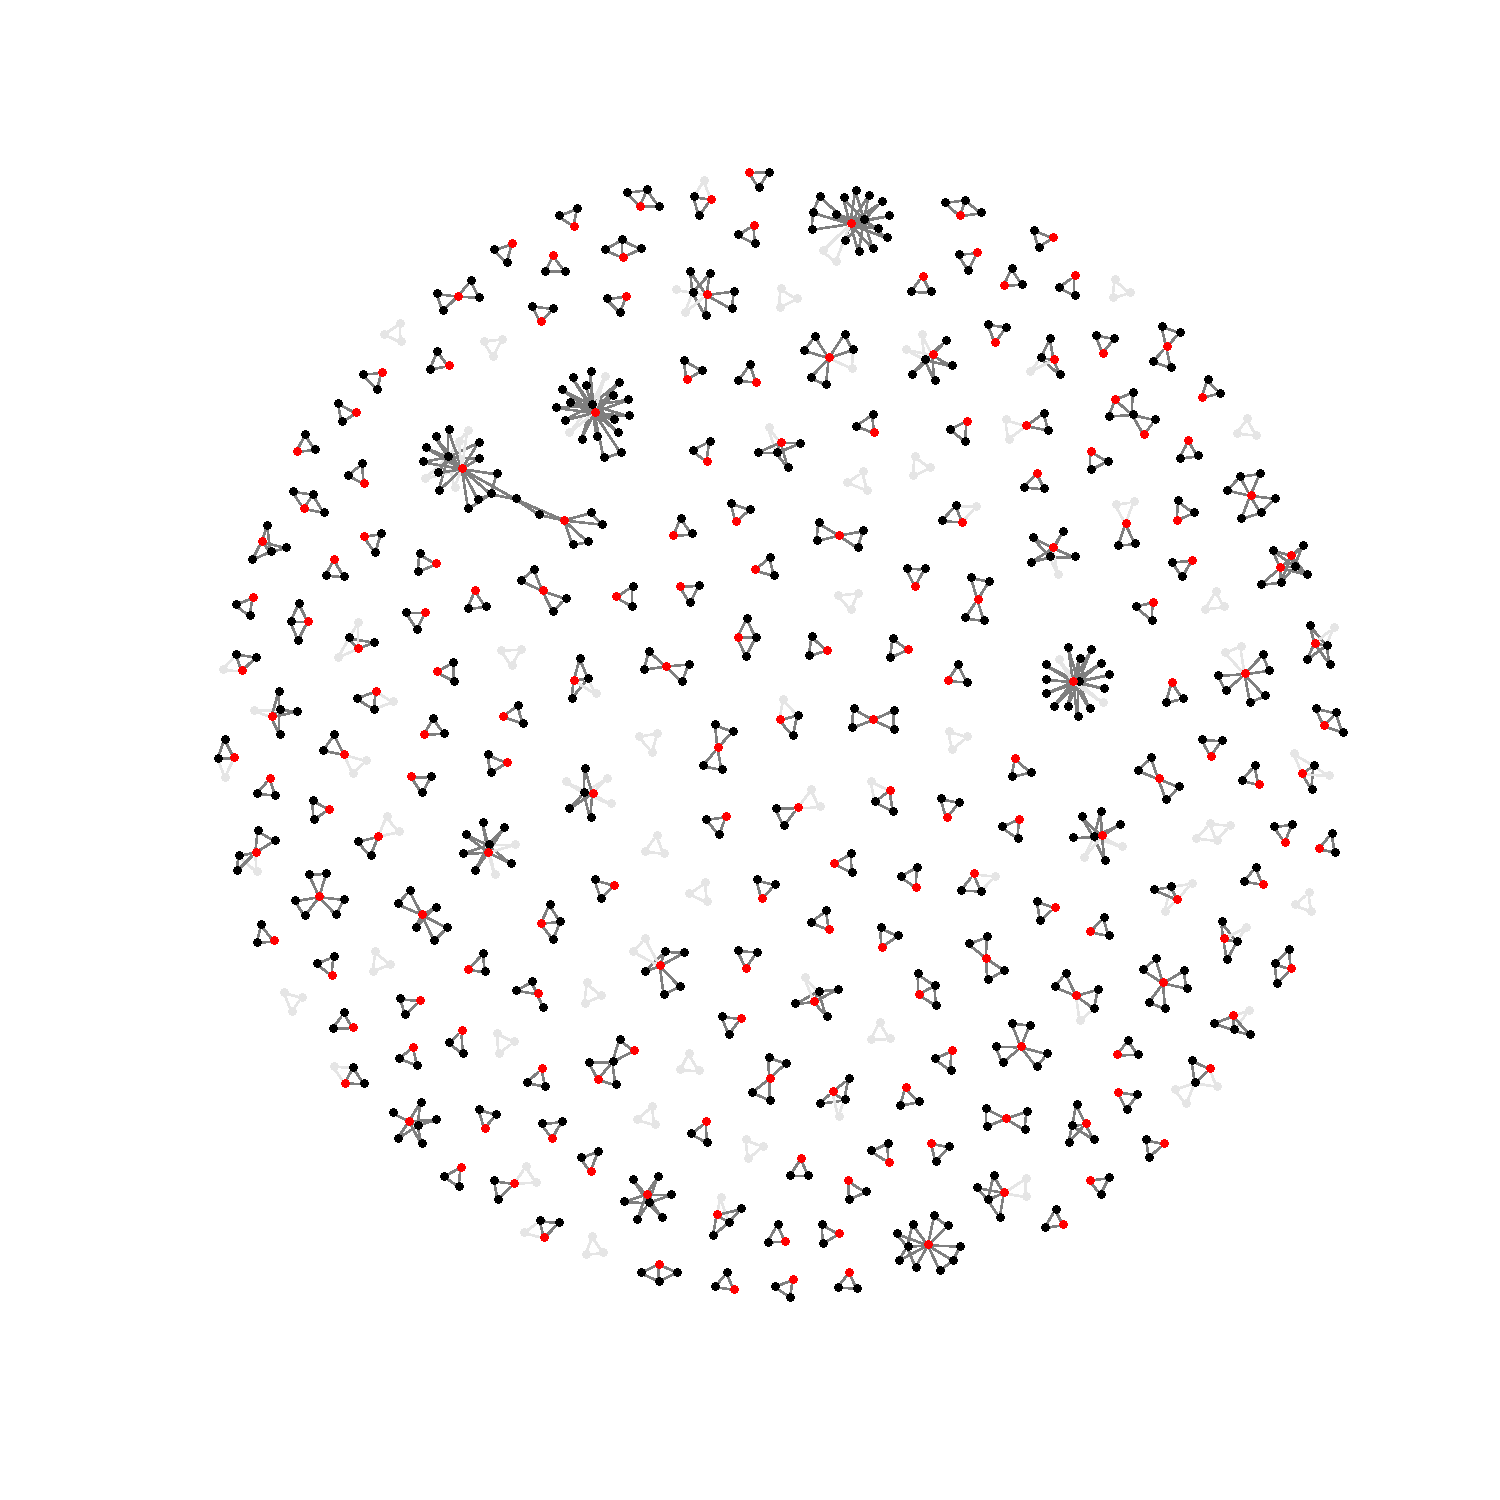
\includegraphics[width=5in]{pale_gray_graph_of_interactions_2_lists_GrayEdges}
	\caption{\textbf{Discovery and replication of epistatic networks} All 434 putative genetic interactions (edges) with data common to discovery and replication sets is shown, where black nodes represent SNPs and red nodes represent traits (gene expression probes). Three hundred and forty-five interactions had $p$-values exceeding the 2.5\% confidence interval following meta analysis of the replication data, but the remaining 89 interactions that did not replicate are depicted in grey. It is evident that a large proportion of the complex networks identified in the discovery set also exist in independent populations.}
	\label{fig:fireworks}
\end{figure}
\clearpage

\begin{figure}[H]
	\centering
	\includegraphics[width=2.5in]{gpbonfrep.pdf}
	\caption{\textbf{Replication of GP maps in two independent populations} The GP maps for each epistatic interaction that is significant at the Bonferroni level in both replication datasets are shown. Each GP map consists of nine tiles where each tile represents the expression level for that two-locus genotype class. Phenotypes are for gene transcript levels (dark coloured tiles = low expression, light coloured tiles = high expression). Columns of GP maps are for each independent population. Rows of GP maps are for each of 30 significantly replicated interactions at the Bonferroni level, corresponding to the rows in Table \ref{tab:bonferroni}. There is a clear trend of the GP maps replicating across all three datasets.}
	\label{fig:gpmaps}
\end{figure}
\clearpage

\begin{figure}[H]
	\centering
	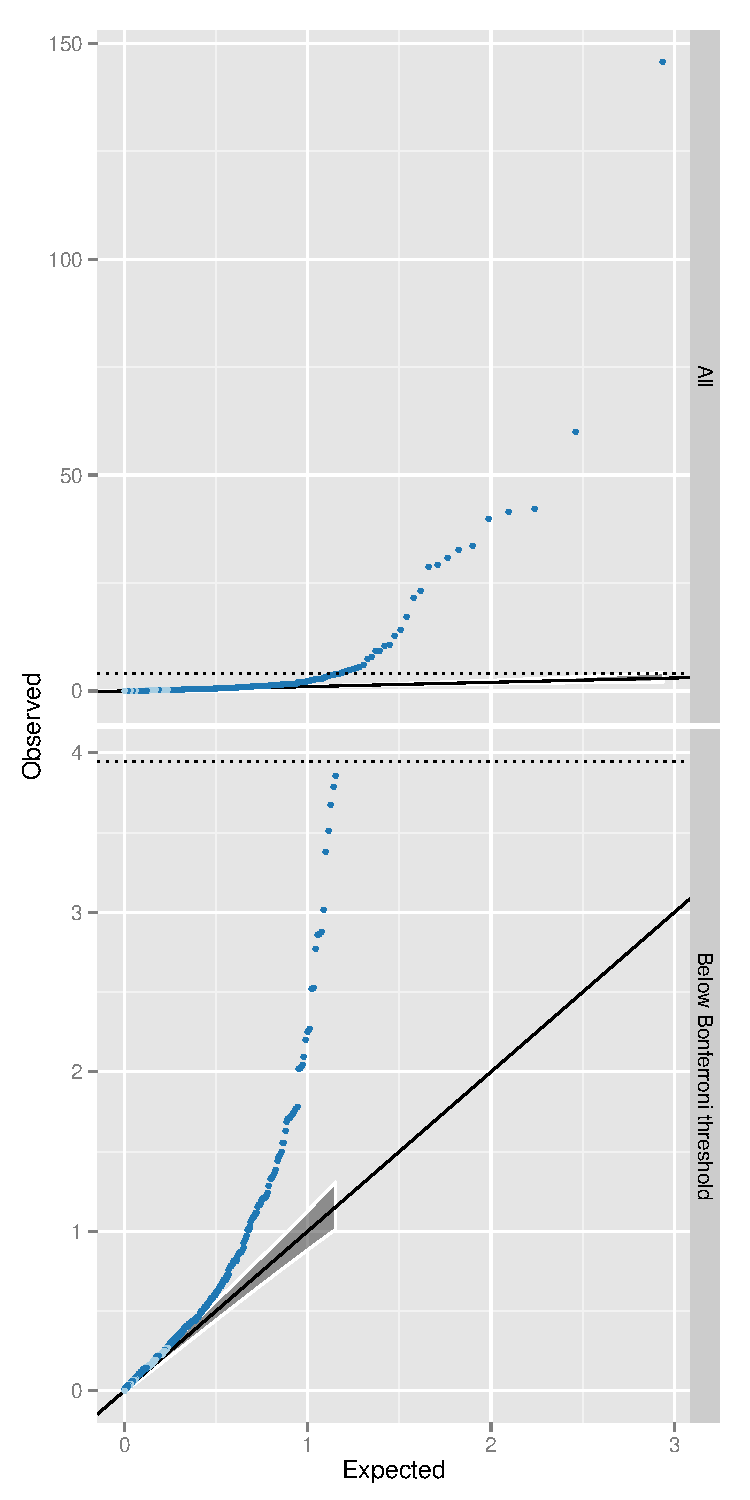
\includegraphics[width=2.5in]{qqMeta.pdf}
	\caption{\textbf{Q-Q plots of interaction $p$-values from replication datasets} The top panel shows all 434 discovery SNPs that were tested for interactions. Observed $p$-values ($y$-axis, $-\log_{10}$ scale) are plotted against the expected $p$-values ($x$-axis, $-\log_{10}$ scale). The multiple testing correction threshold for significance following Bonferroni correction is denoted by a dotted line. The bottom panel shows the same data as the top panel but excluding the 30 interactions that were significant at the Bonferroni level in the replication datasets. The shaded grey area represents the 5\% confidence interval for the expected distribution of $p$-values. Dark blue points represent $p$-values that exceed the confidence interval, light blue are within the confidence interval.}
	\label{fig:qqMeta}
\end{figure}
\clearpage


\clearpage
\section{Supplementary Figures}
\setcounter{figure}{0}
\makeatletter 
\renewcommand{\thefigure}{S\@arabic\c@figure} 
\makeatletter 


\begin{figure}[H]
	\centering
	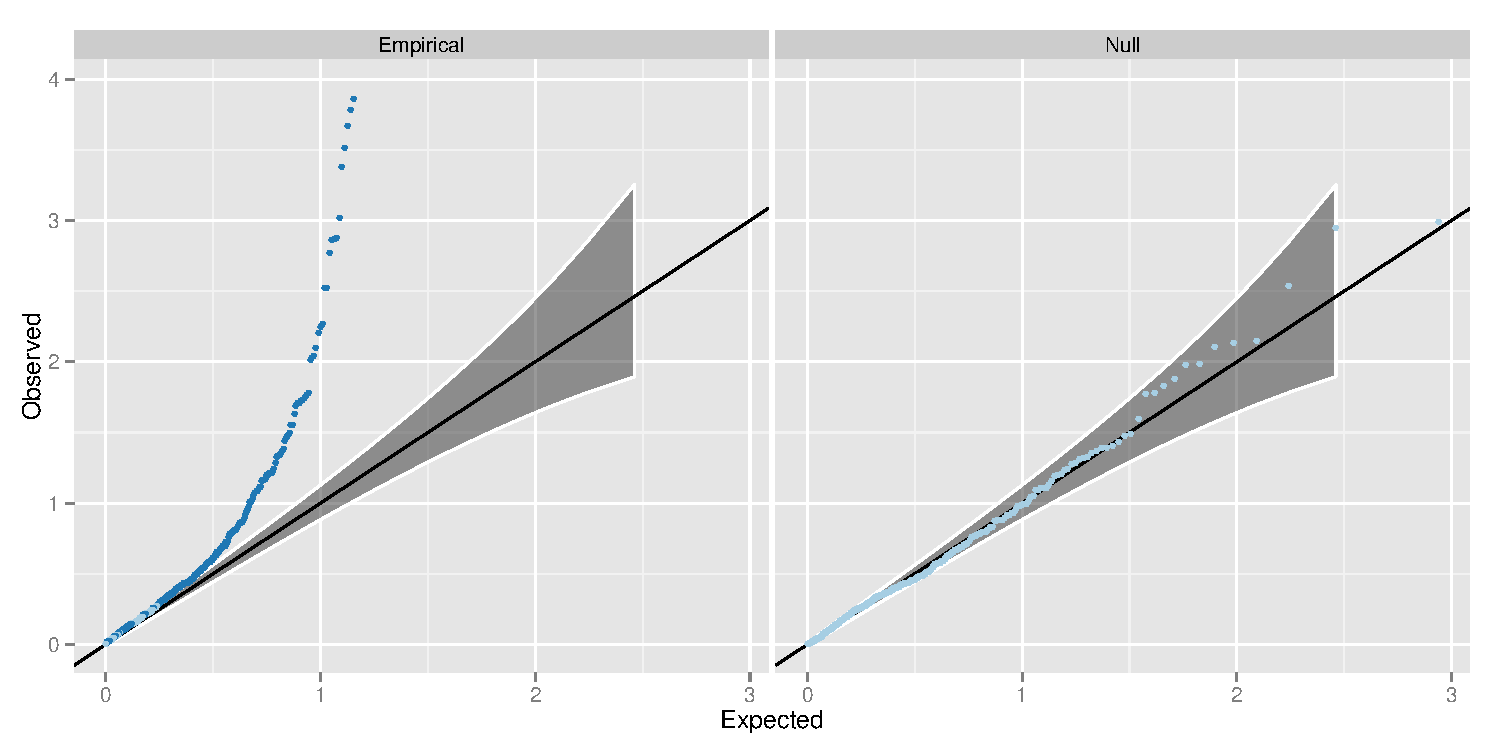
\includegraphics[width=5in]{qqMetaNonsig}
	\caption{\textbf{Q-Q plots of interaction $p$-values from replication datasets, excluding the 30 points significant at the Bonferroni level} The right panel (Null) shows the interaction $p$-values from a meta analysis across two independent datasets on 434 randomly drawn SNP pairs. The left panel (Empirical) shows the interaction $p$-values from the 404 putative interactions that were not significant at the Bonferroni correction threshold. Dark blue points represent $p$-values that surpass the 2.5\% FDR level, as in Figure \ref{fig:qqMeta}.}
\label{fig:qqMetaNonsig}
\end{figure}
\clearpage

\begin{figure}
	\centering
	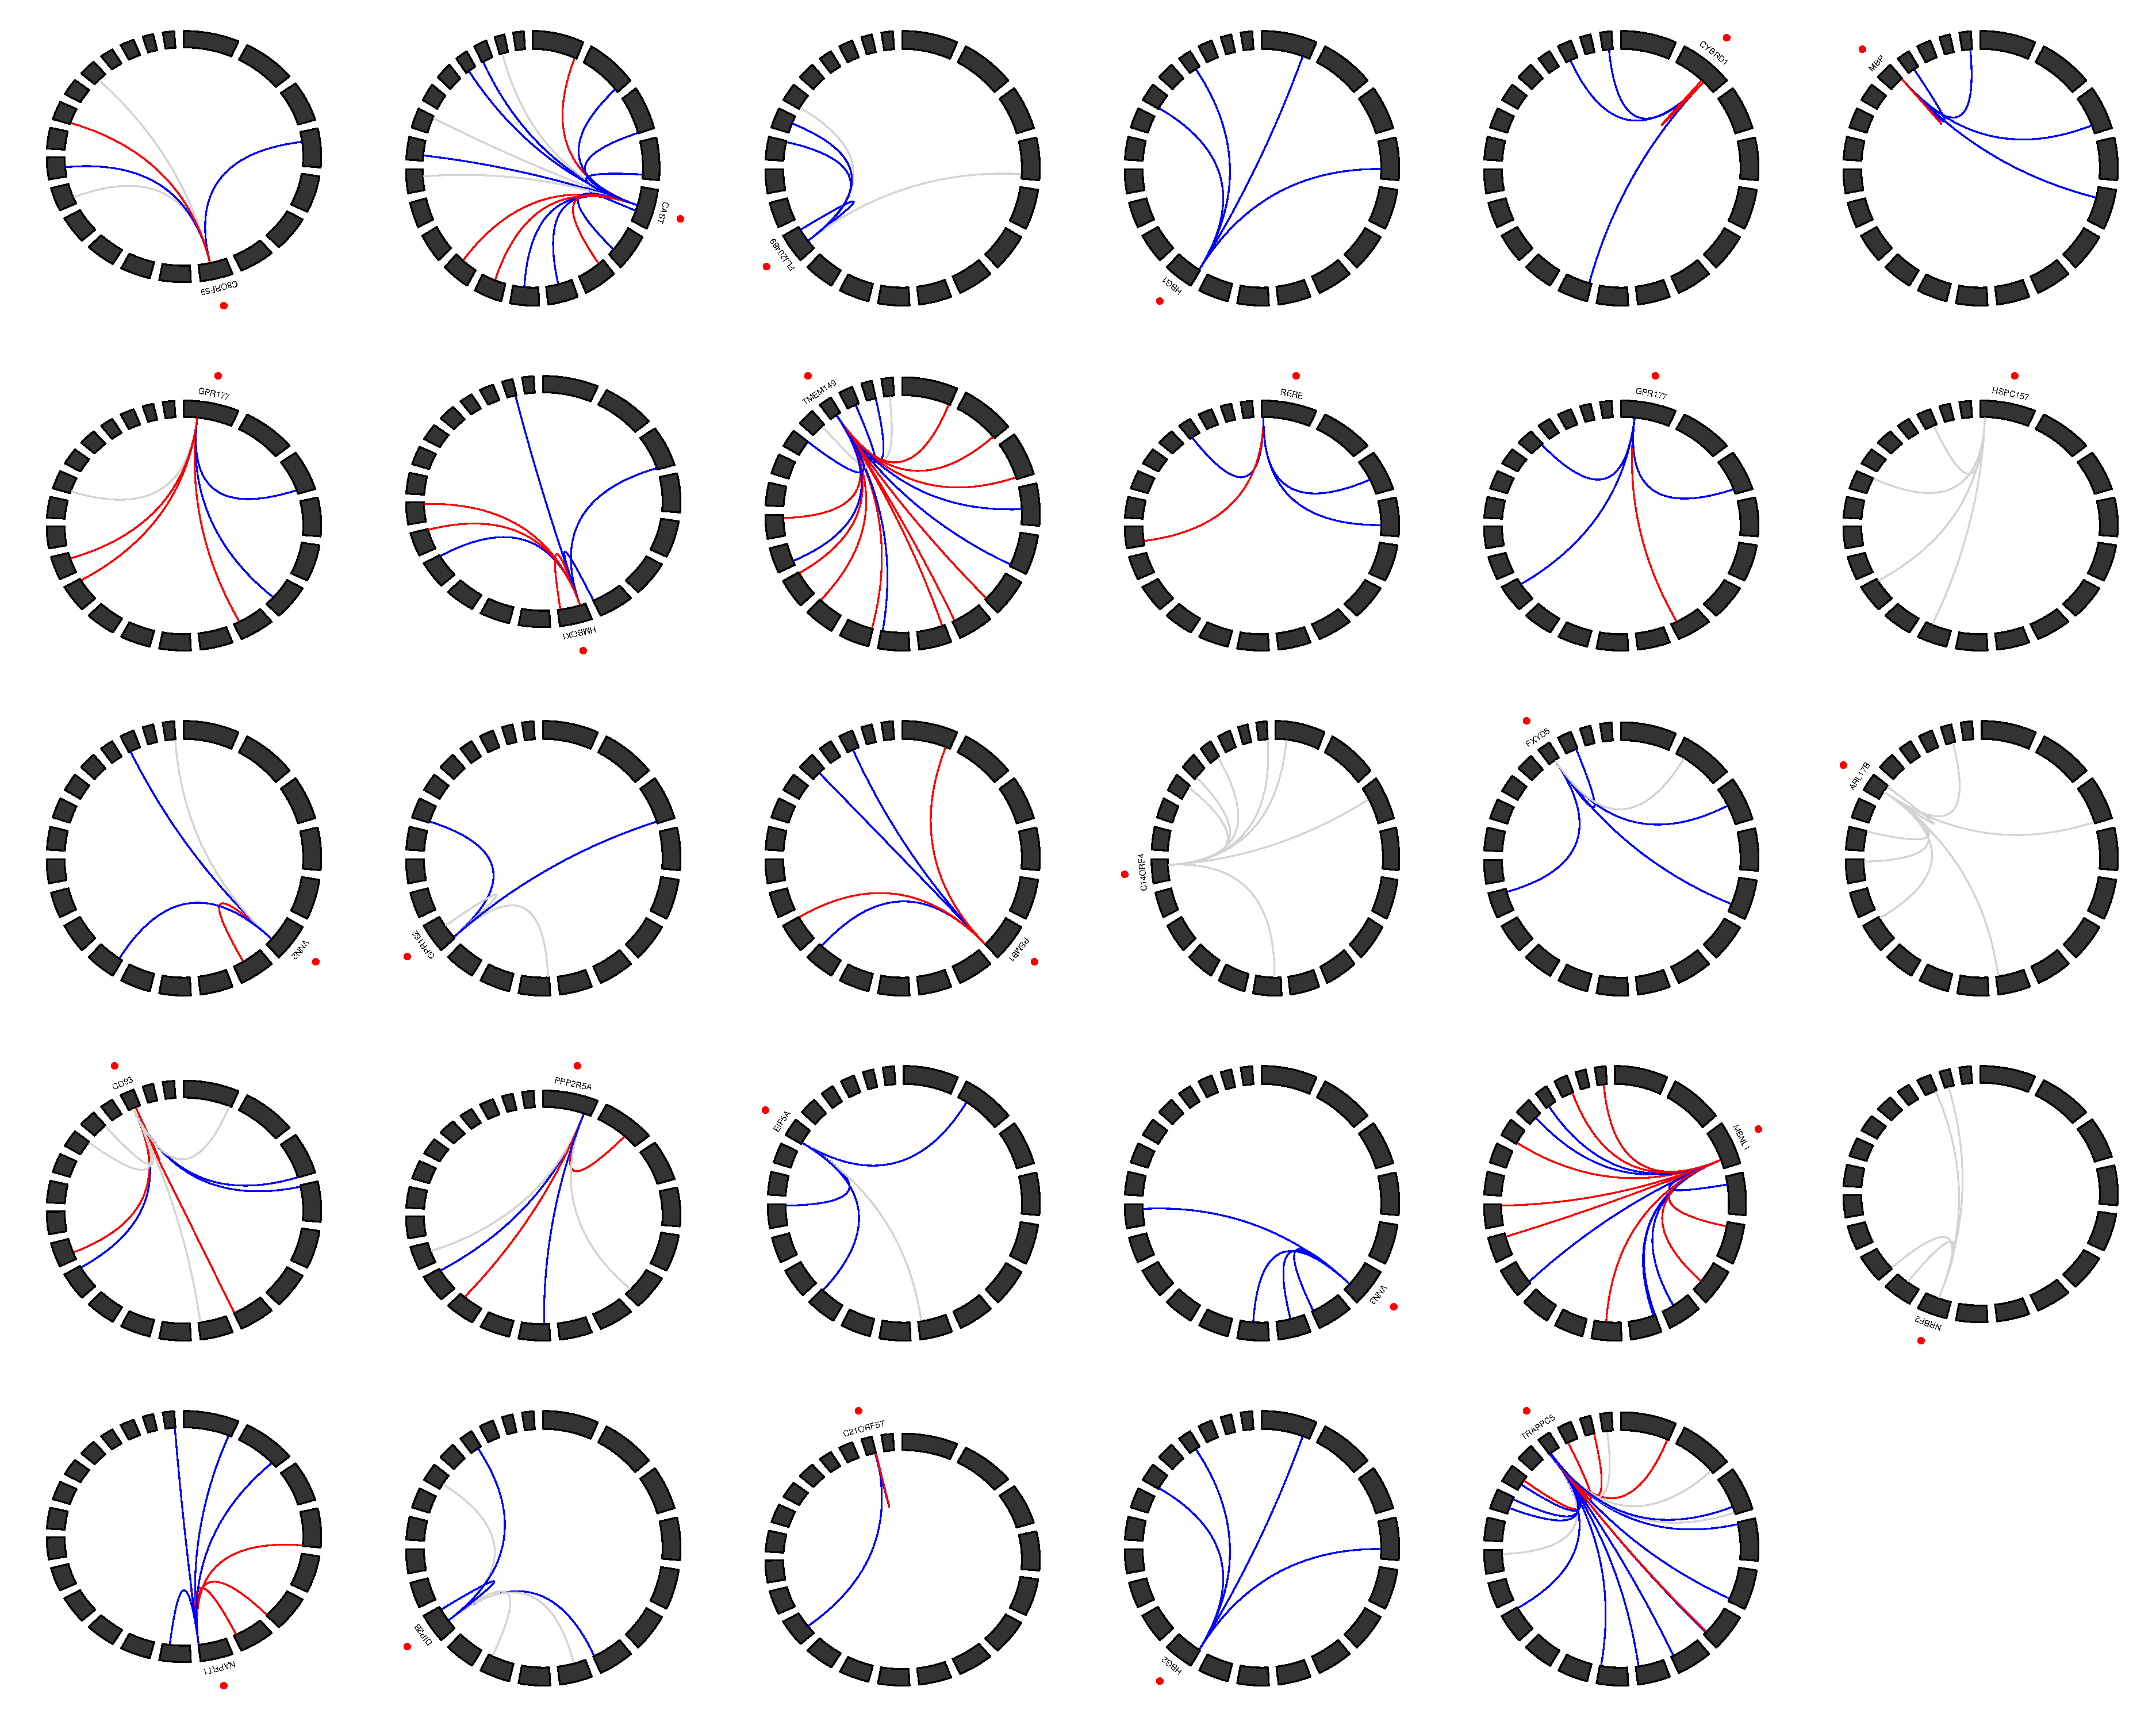
\includegraphics[width=5in]{circles_replication2}
	\caption{\textbf{Gene expression traits with four or more genetic interactions} Circle plots represent the genomic positions for SNPs (linking lines) and expression probes (red points). Chromosomes are represented by black blocks and ordered from 1 to 22 clockwise, starting from the top. Grey lines represent no evidence for replication, blue lines denote replication in at least one dataset, and red lines denote replication in two datasets. Most interactions are characterised as being \emph{cis}-\emph{trans} to the expression probe.}
	\label{fig:circleplots}
\end{figure}
\clearpage

\begin{figure}
	\centering
	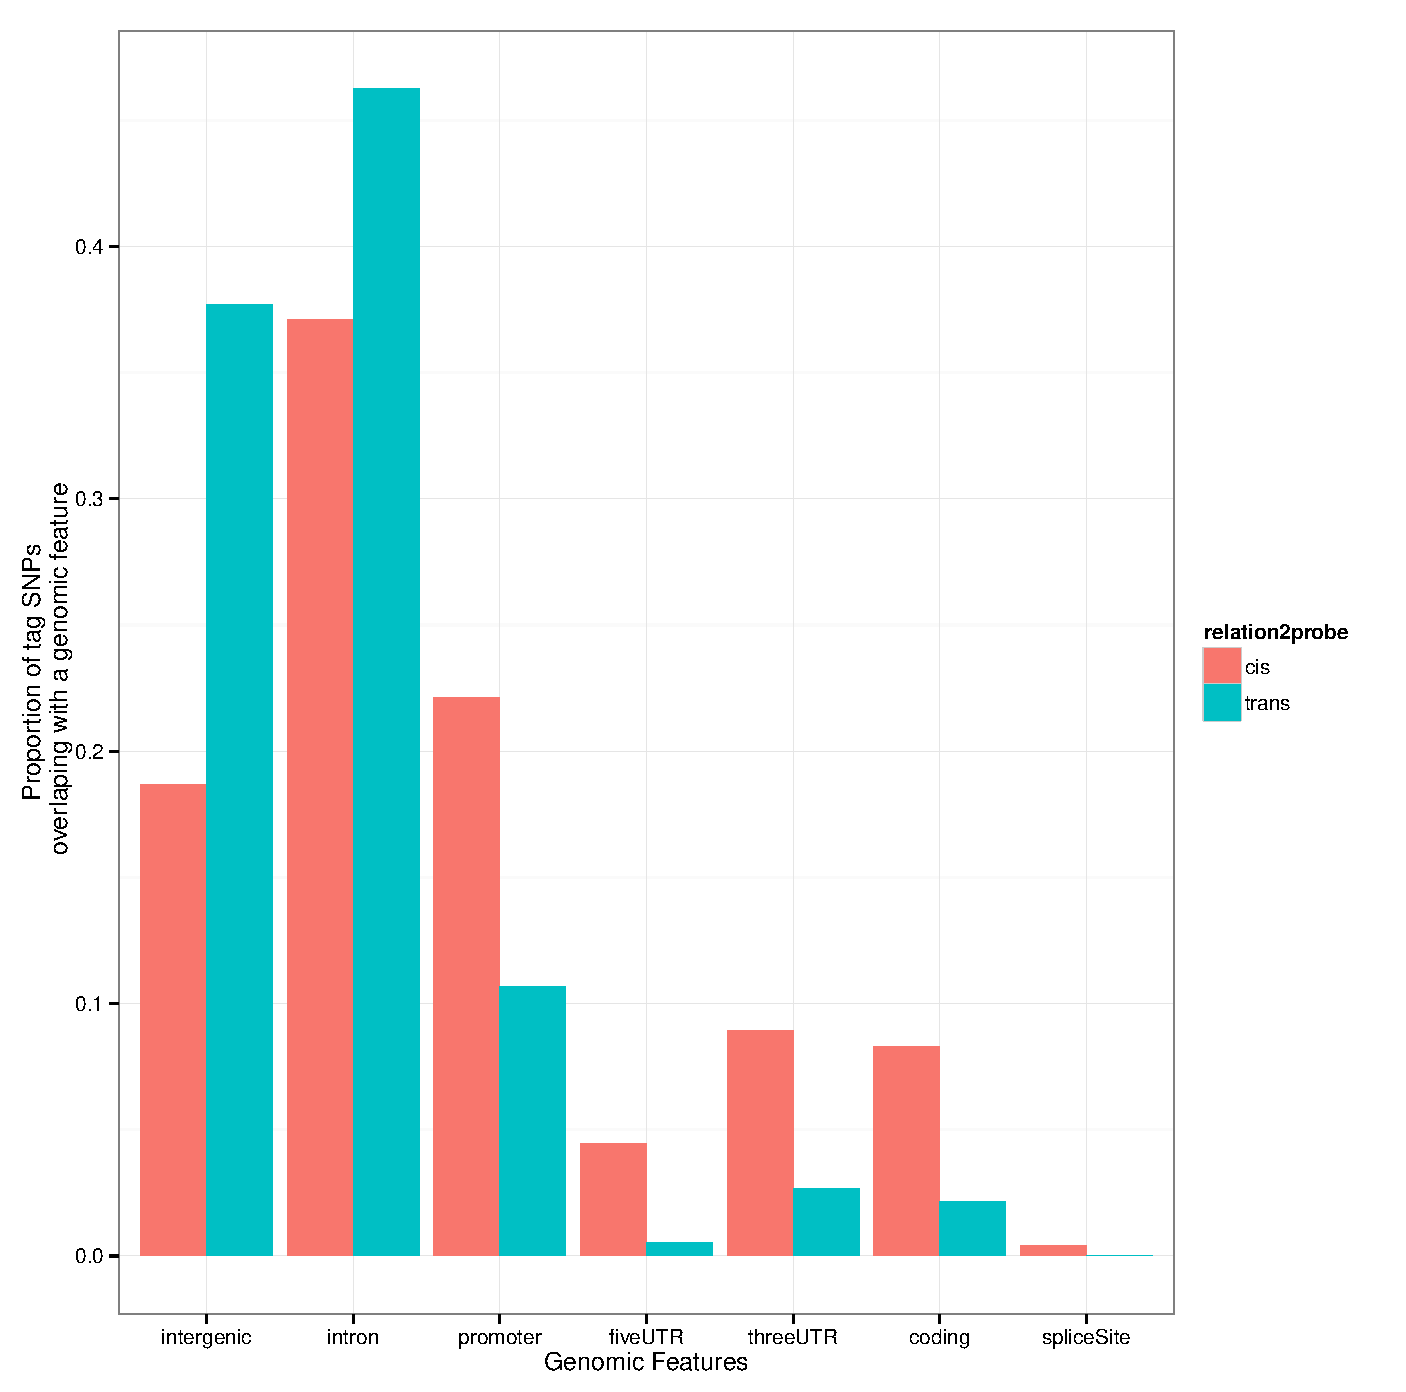
\includegraphics[width=5in]{OverlapAnnotation}
	\caption{\textbf{Location of SNPs relative to genomic features} All SNPs within 5kb and $r^2 > 0.8$ of each \emph{cis}- and \emph{trans}-SNP were taken to find which genomic regions were covered by the 501 significant interactions. There is enrichment for \emph{cis}-acting SNPs in promotor regions, and \emph{cis}- and \emph{trans}-acting SNPs in intronic regions.}
	\label{fig:snplocations}
\end{figure}
\clearpage

\begin{figure}
	\centering
	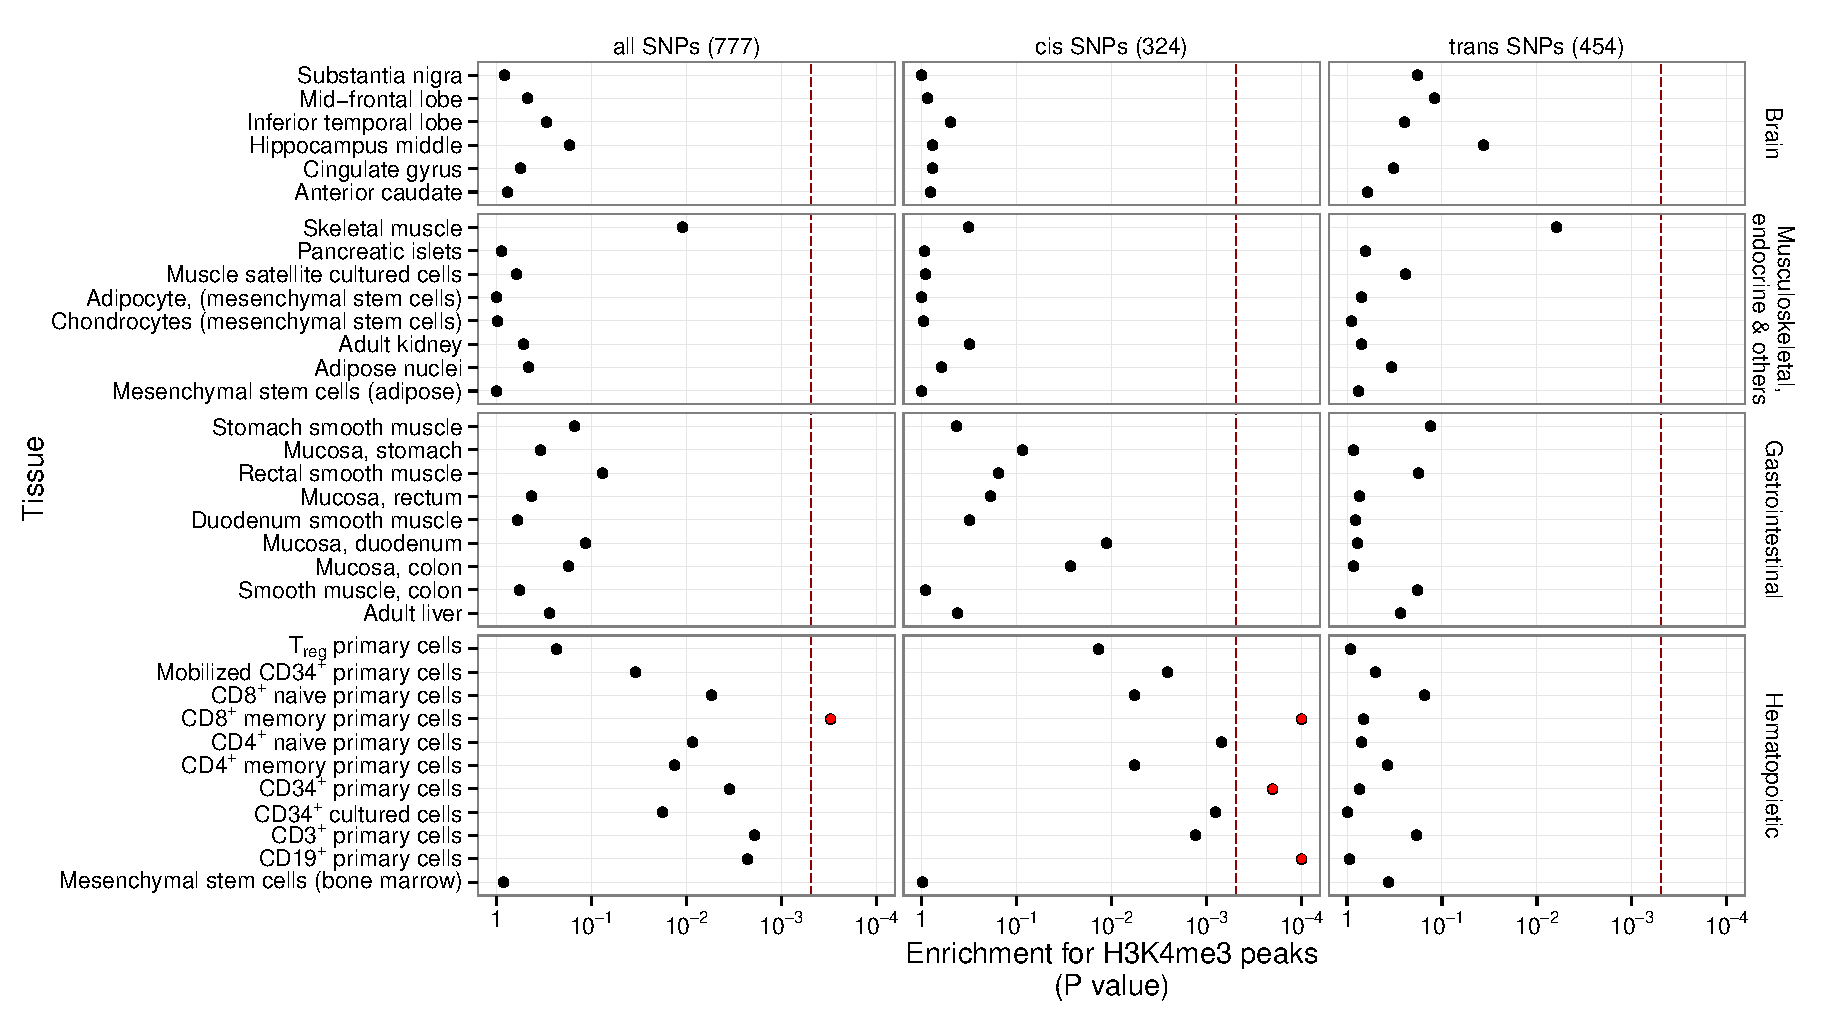
\includegraphics[width=5in]{501_pairs_snp_list_Grid}
	\caption{\textbf{Tissue specific enrichment of SNPs in transcriptionally active regions} The locations of transcriptional activity can be predicted by chromatin marks, assayed by H3K4me3 \cite{Trynka2013}. Enrichment $p$-values are calculated using permutation analysis for 34 different cell types ($y$-axis) in four tissue types (Rows of boxes). There is enrichment for \emph{cis}-acting SNPs in Haematopoietic tissue types only. \emph{Trans}-acting SNPs have no tissue specificity.}
	\label{fig:h3k4me3}
\end{figure}
\clearpage

\begin{figure}
	\centering
	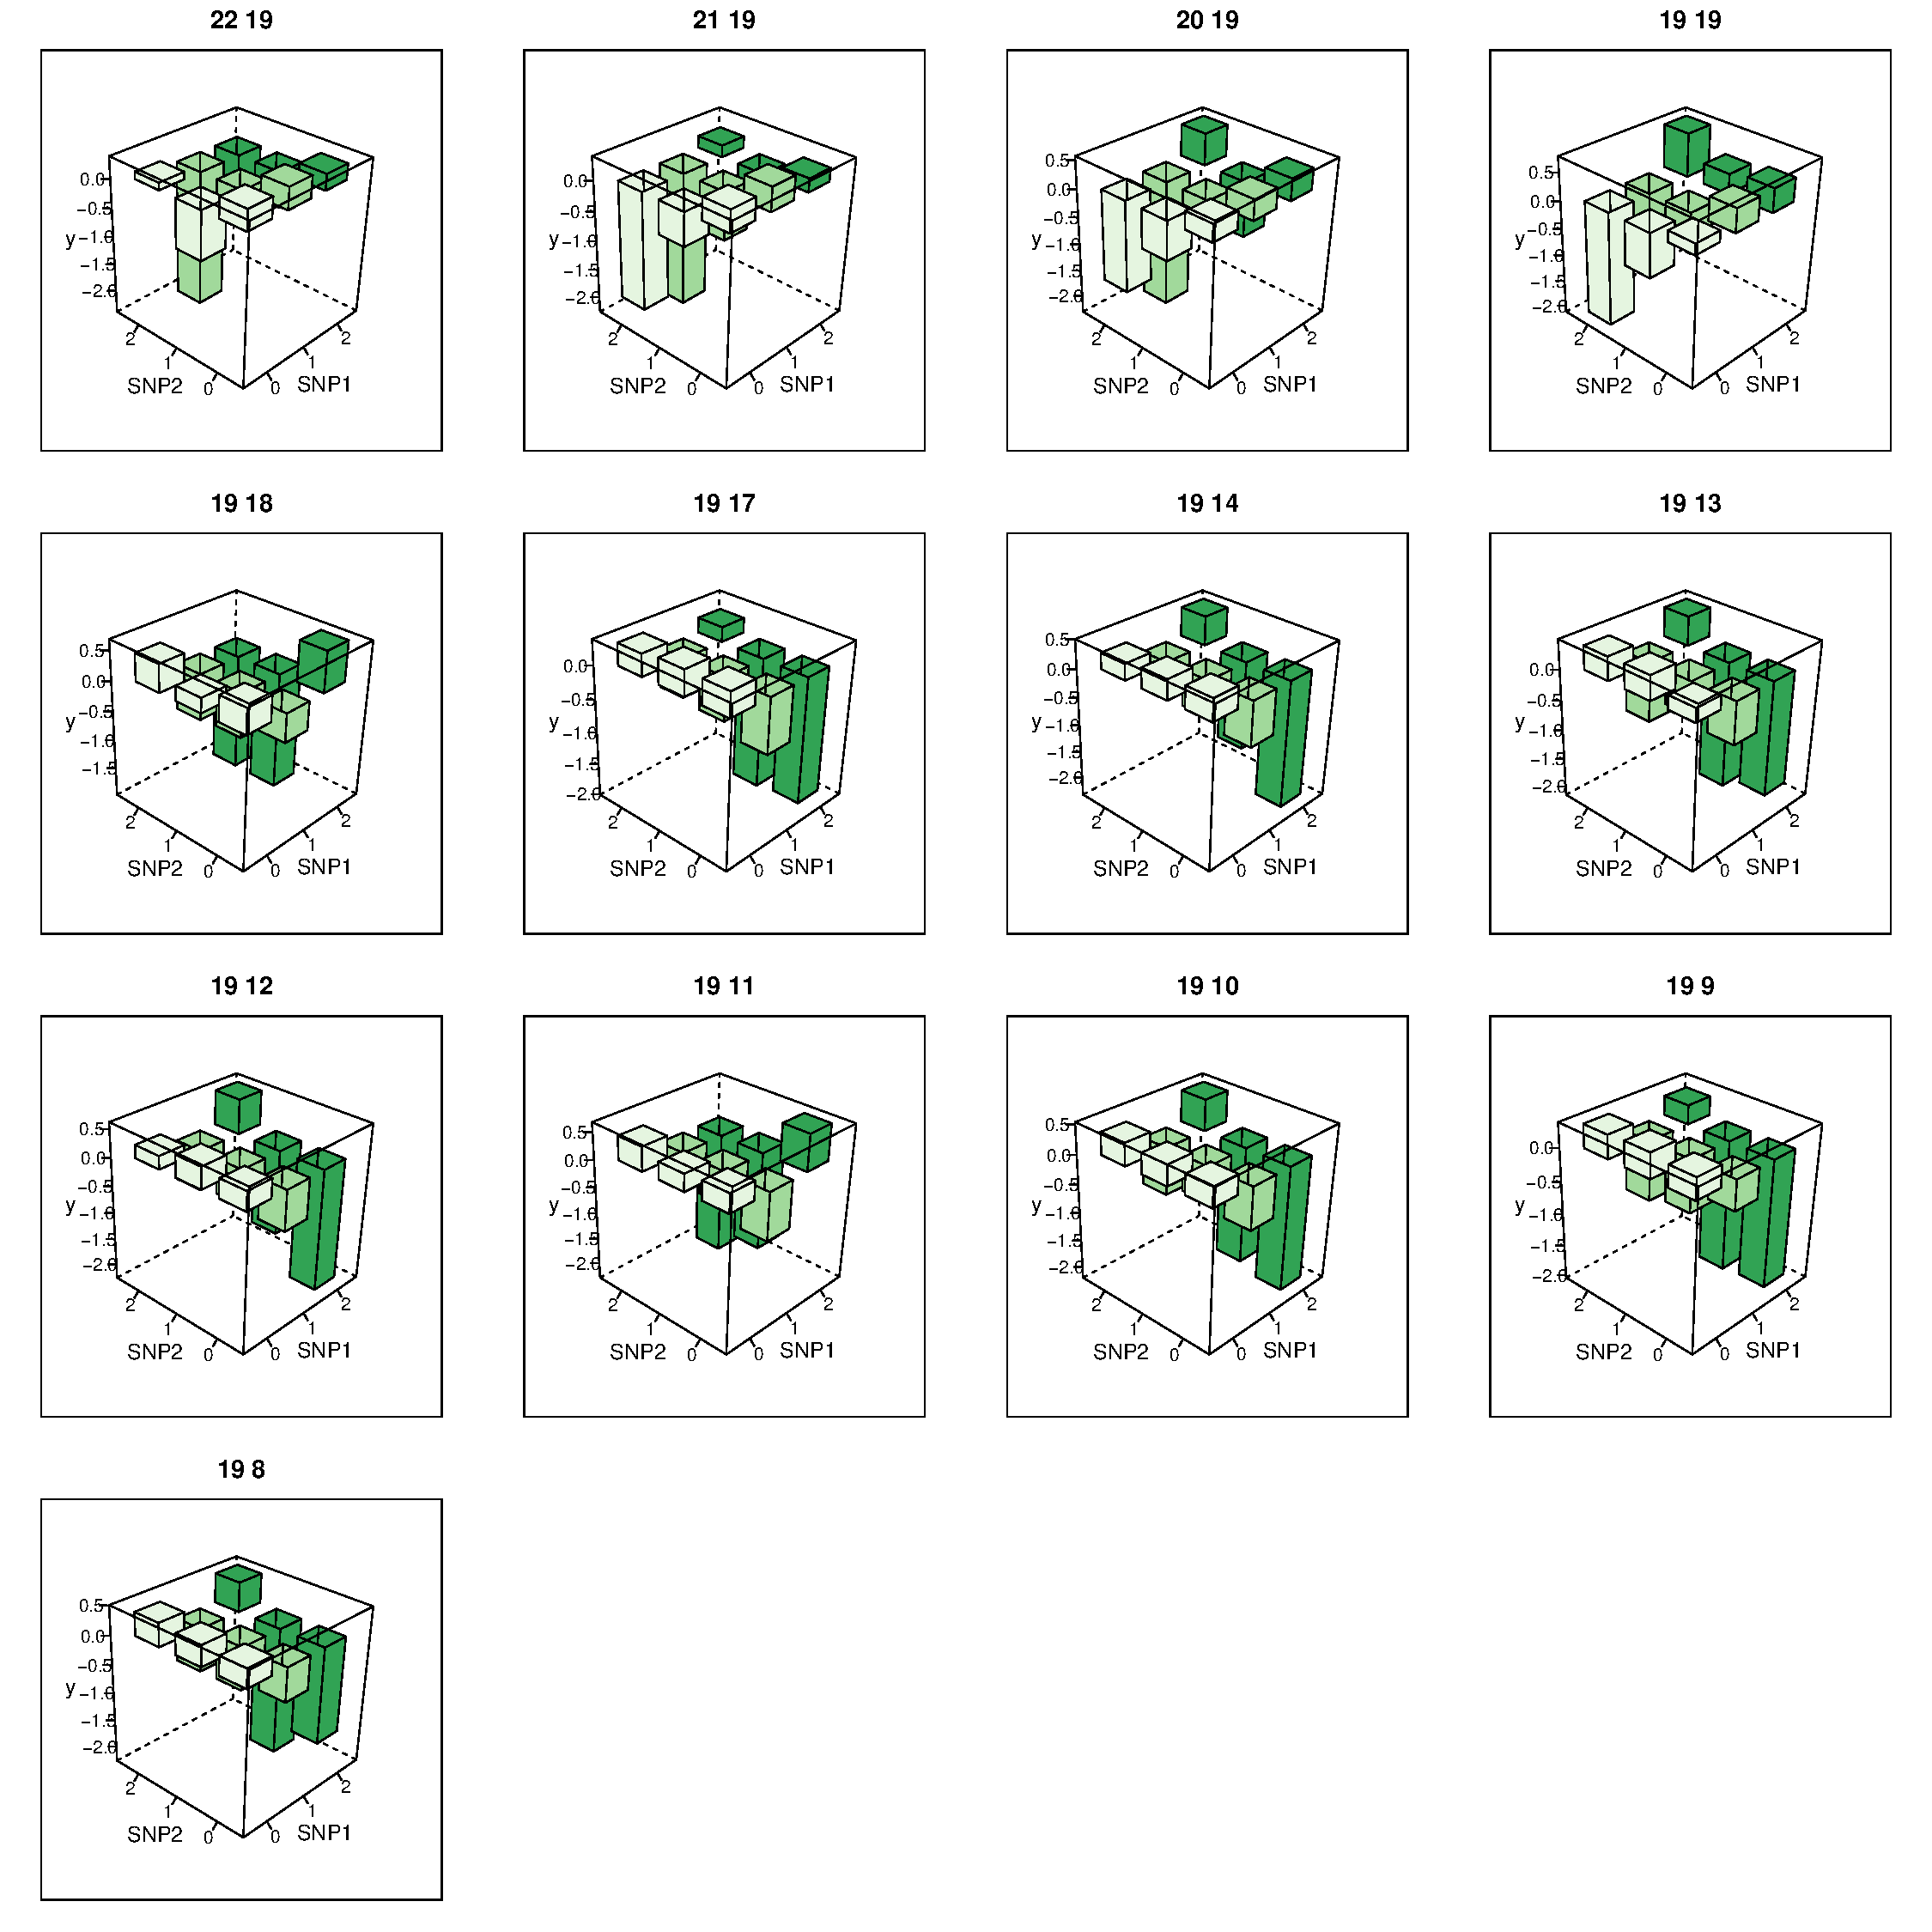
\includegraphics[width=5in]{MBNL1}
	\caption{\textbf{Genotype-phenotype maps for 14 interactions controlling MBNL1} Each bar represents the mean phenotypic value for individuals in that genotype class. The rs13069559 SNP typically has a \emph{cis}-additive decreasing effect on the expression of MBNL1, but in many of these interactions the \emph{cis} effect is masked when the \emph{trans} SNP is homozygous.}
	\label{fig:mbnl13d}
\end{figure}
\clearpage

\begin{figure}
	\centering
	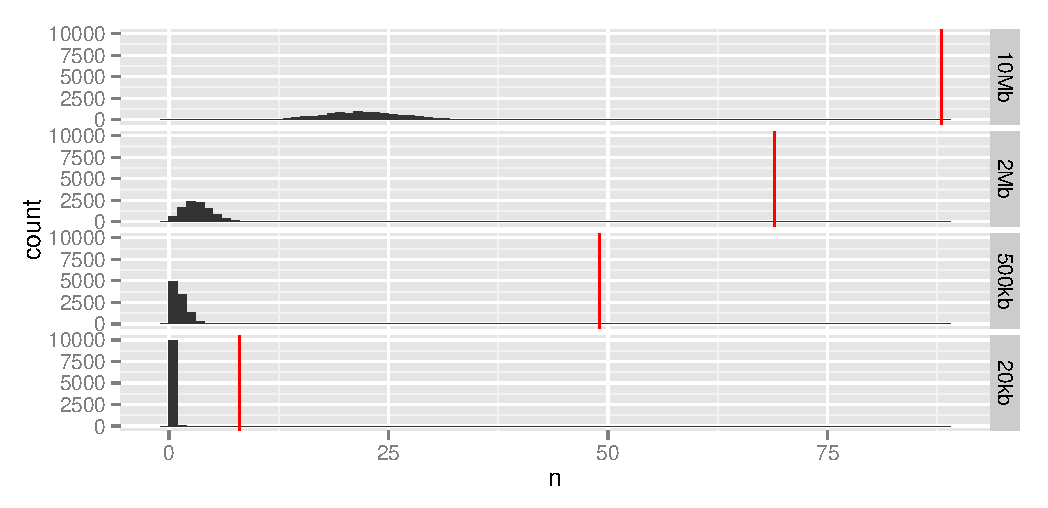
\includegraphics[width=5in]{chromosome_interactions}
	\caption{\textbf{Number of overlaps between chromosome interactions and epistatic interactions} Interacting chromosome regions may be a possible mechanism underlying epistatic interactions. The number of epistatic interactions within 20kb, 500kb, 2Mb and 10Mb of known chromosome interacting regions are shown by red vertical lines. The histograms represent the null distribution based on random sampling of 10,000 datasets for each window size.}
	\label{fig:chromosomeinteractions}
\end{figure}
\clearpage

\begin{figure}
	\centering
	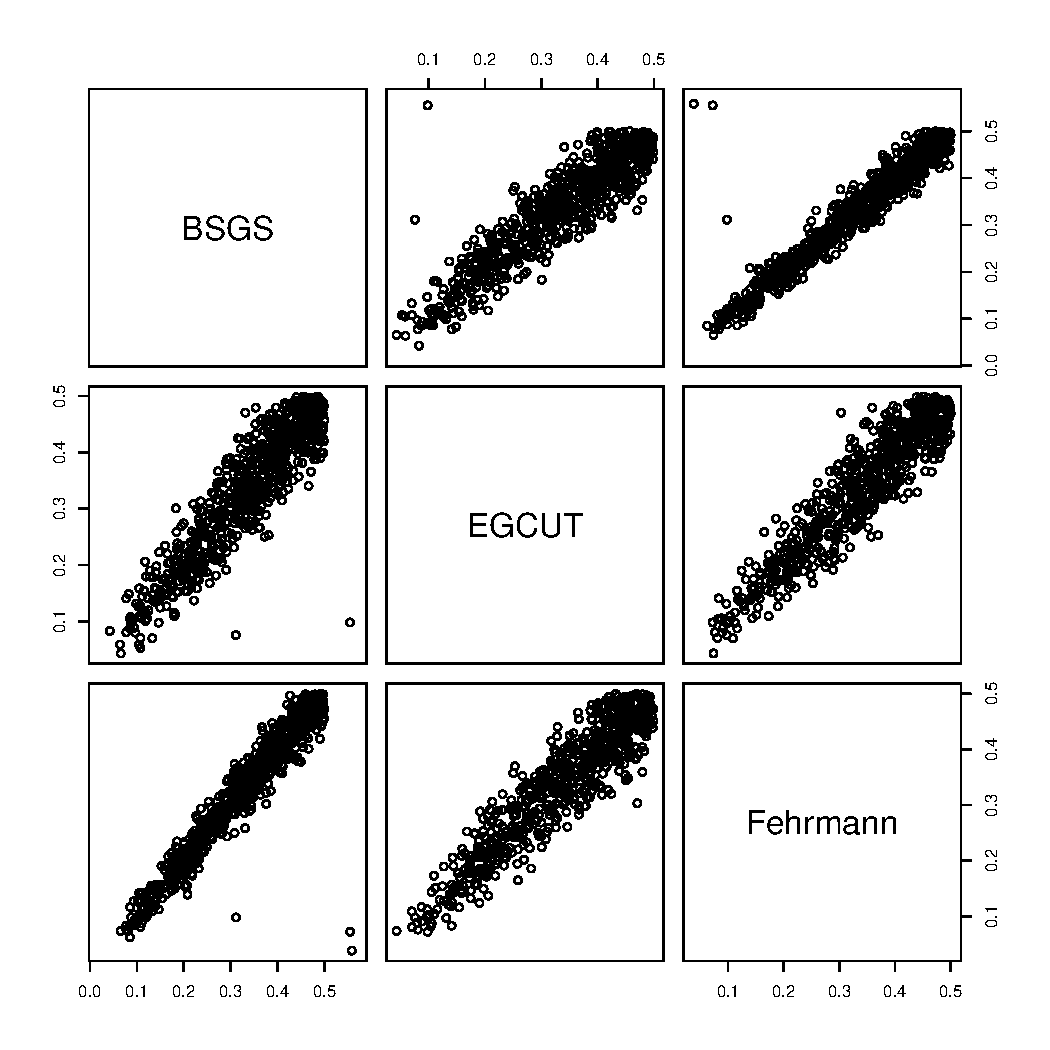
\includegraphics[width=5in]{alleleFreq}
	\caption{\textbf{Comparison of allele frequencies for 781 SNPs involved in genetic interactions across independent populations} Outliers were removed from the analysis as part of the filtering stage during replication.}
	\label{fig:allelefreq}
\end{figure}




\clearpage
\section{References}
\bibliography{refs}

\end{document}